\documentclass[10pt,a4paper]{article}
\usepackage[utf8x]{inputenc}
\usepackage{ucs}
\usepackage[spanish]{babel}
\usepackage[left=2cm,top=4cm,right=2cm,bottom=3cm]{geometry} 
\usepackage{amsmath}
\usepackage{amsfonts}
\usepackage{amssymb}
\usepackage{dcolumn}
\usepackage{float}
\usepackage{graphicx}
\usepackage{ esint }
\usepackage{fancyhdr}
\usepackage{enumerate} 
\pagestyle{fancy}
\usepackage{tocbibind}
\usepackage{setspace}
\usepackage{parskip}
\usepackage[hidelinks]{hyperref}
\usepackage{listings}    
\usepackage[titletoc,toc,page]{appendix}
\usepackage{pdfpages}
\renewcommand{\appendixtocname}{Anexo}
\renewcommand{\appendixpagename}{Anexo}
\lhead{Proyecto Final }
\rhead{
\includegraphics[width=1.5 cm]{logo}}
\author{cyn}
\begin{document}
\begin{titlepage}
\begin{center}
\vspace*{-1in}
\begin{figure}[htb]
\begin{flushleft}

\includegraphics[width=5cm]{./logo}
\end{flushleft}
\end{figure}
\begin{LARGE}
\textbf{U.B.A. FACULTAD DE INGENIERÍA}\\
\end{LARGE}
\vspace*{0.15in}
\begin{LARGE}
\textbf{Departamento de Electrónica}\\
\end{LARGE}
\vspace*{0.2in}
\begin{LARGE}
\textbf{Organización de computadoras 66-20}\\
\end{LARGE}
\vspace*{0.2in}
\begin{Large}
\textbf{TRABAJO PRÁCTICO \#0}\\
\end{Large}
\vspace*{0.2in}
\begin{LARGE}
\textit{Infraestructura básica }\\
\end{LARGE}
\vspace*{0.2in}
\begin{Large}
\raggedright\textbf{Curso: 2018 - 2do Cuatrimestre}\\
\end{Large}
\vspace*{0.1in}
\begin{Large}
\raggedright\textbf{Turno: Martes}\\
\end{Large}
\vspace*{0.1in}

\begin{table}[htb]
\begin{center}
\begin{spacing}{1.9}
\begin{tabular}{| l | l |}
\hline
\multicolumn{2}{|>{\arraybackslash}p{15cm}|}{\begin{Large}
\textbf{GRUPO N°}
\end{Large}}\\
\hline
\textbf{Integrantes} & \textbf{Padrón} \\
\hline
\makebox[8cm][c]{Verón, Lucas} & \makebox[2.5cm][c]{89341}\\
\hline
\makebox[8cm][c]{Gamarra Silva, Cynthia Marlene} & \makebox[2.5cm][c]{92702}\\
\hline
\makebox[8cm][c]{Gatti, Nicolás} & \makebox[2.5cm][c]{88888}\\
\hline
\textbf{Fecha de entrega: } & \hspace{0.8cm}23-11-2018\\
\hline
\textbf{Fecha de aprobación: } & \\
\hline
\textbf{Calificación: } & \\
\hline
\textbf{Firma de aprobación:} & \\
\hline
\end{tabular}
\end{spacing}
\end{center}
\end{table}
\fbox{%
\begin{minipage}[c][3.4cm][l]{.9\linewidth}
\textbf{Observaciones:} \\
\vfill
\end{minipage}
}
\end{center}

\vspace*{0.1in}
\end{titlepage}
\tableofcontents 
\vspace*{0.3in}
\newpage

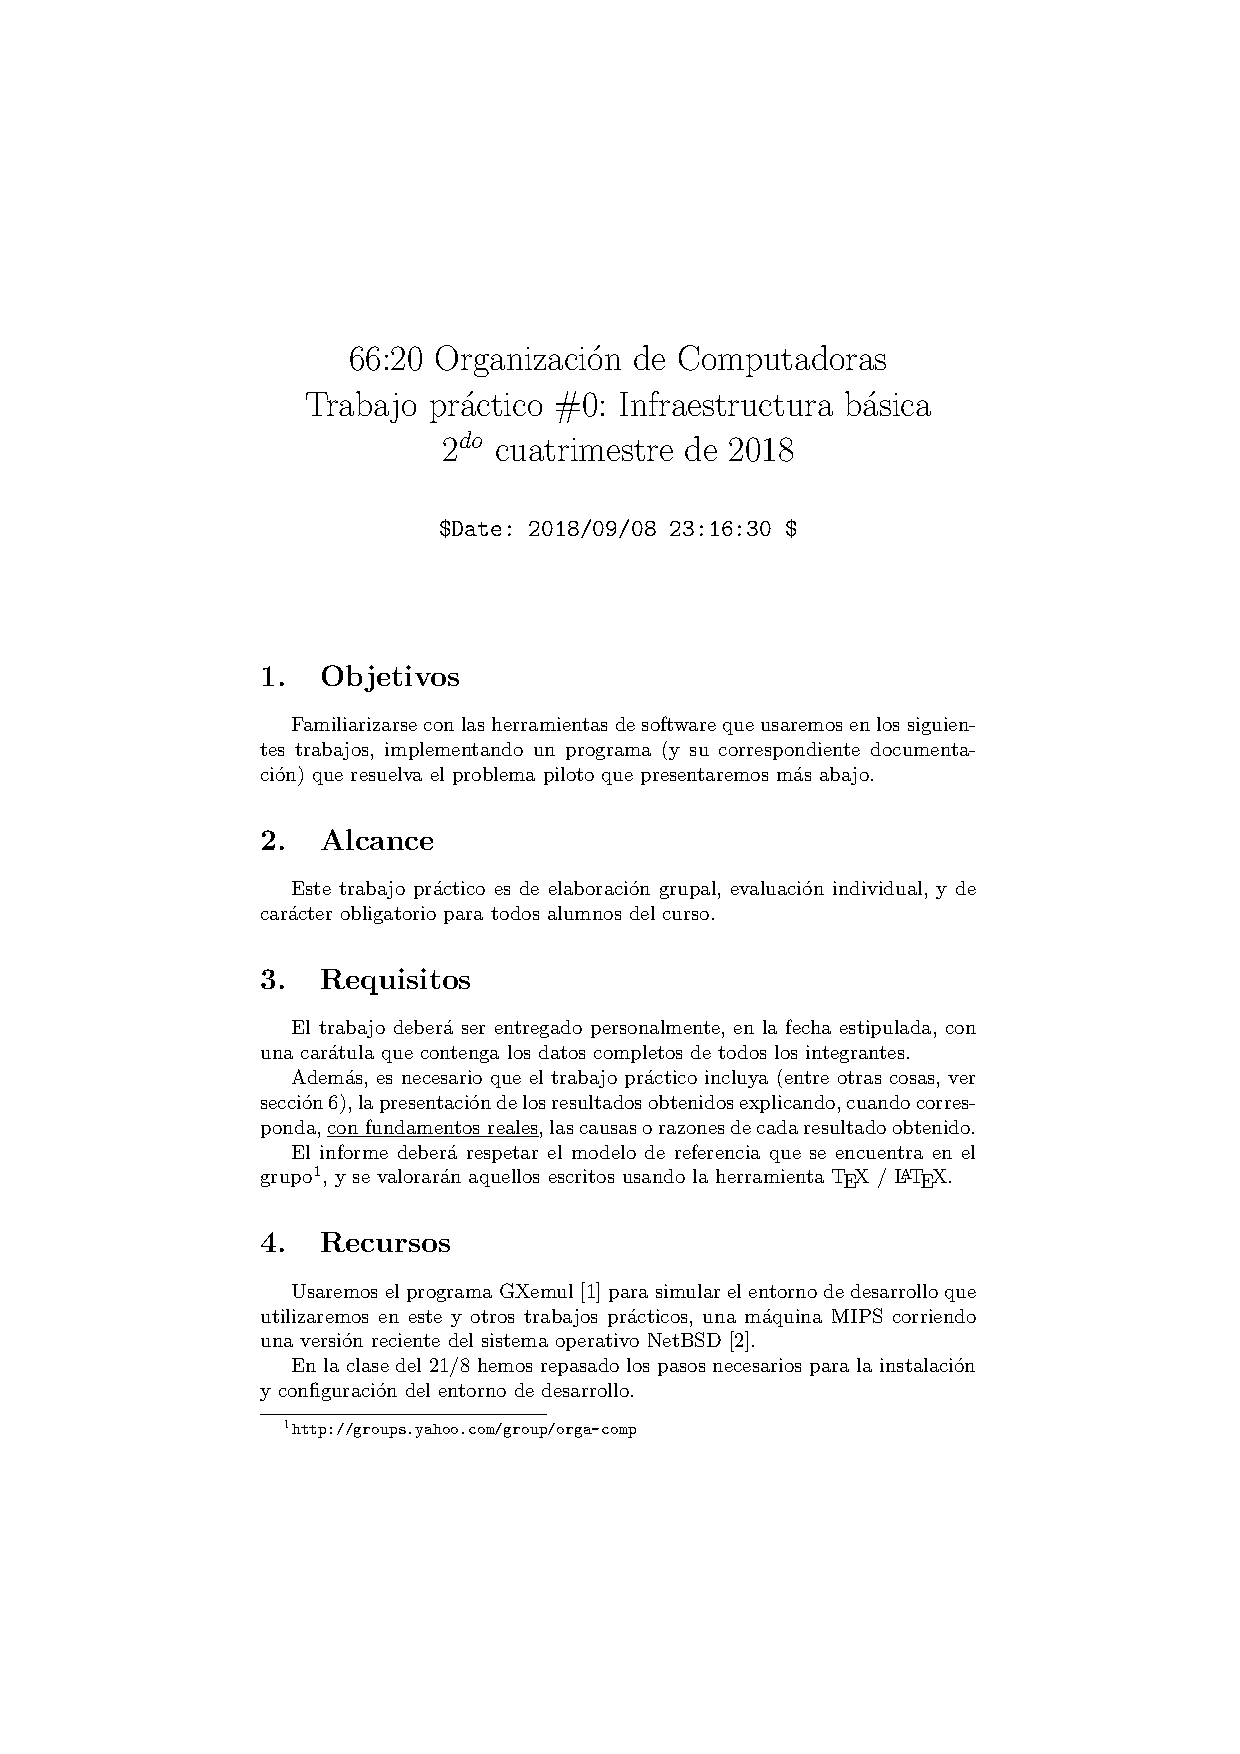
\includepdf[pages=1,scale=0.95,pagecommand = \section{Enunciado del trabajo práctico}\label{enunciado},offset=10 -10]{../tp0-2018-2q.pdf}
\includepdf[pages={2-last},scale=0.95,pagecommand = {},offset=10 -10]{../tp0-2018-2q.pdf}


\section{Objetivos}


\newpage
\section{Desarrollo}


 \newpage

\subsection{Diseño e implementación}

\newpage

\subsection{Compilación del programa}

\newpage

\section{Pruebas realizadas}

\newpage


\begin{thebibliography}{10}
	%	\bibitem{book_CompArch} Hennessy, J. L. - Patterson, D. A. - \emph{Computer Architecture: A Quantitative Approach} - 3\textsuperscript{rd} edition - Morgan Kaufmann - 2002.
	%	\bibitem{book_CompOrg} Patterson, D. A. - Hennessy, J. L. - \emph{Computer Organization and Design: The Hardware/Software Interface} - 3\textsuperscript{rd} edition - Morgan Kaufmann - 2004.
	\bibitem{book_Cprogr} Kernighan, B. W. - Ritchie, D. M. - \emph{C Programming Language} - 2\textsuperscript{nd} edition - Prentice Hall - 1988.
	\bibitem{gnu_make} \emph{GNU Make} - \hyperlink{make}{https://www.gnu.org/software/make/}
	\bibitem{valgrind} \emph{Valgrind} - \hyperlink{valgrind}{http://valgrind.org/}

\end{thebibliography}

%-----------------------------------%
%									%
%			Seccion:Fuente			%
%									%
%-----------------------------------%
\appendix
\section{Código fuente}\label{appendix_codigo_fuente}

\subsubsection{main.c}\label{main}
%\lstinputlisting[language=C, style=StyleC]{main.c}

\newpage




\end{document}
